
% SUBMITTED VERSION:
% Generally, research in Language \& Vision (L\&V) is interested in modeling how speakers naturally talk about visual objects and scenes, in contrast to the fixed image labeling schemes used in Computer Vision.
% Data collections in L\&V are typically set up as free annotation tasks,  where subjects are free to produce whatever word or utterance they consider most suitable for the given task (e.g.\ image description, reference to objects, visual dialogue), which naturally results in linguistic variation.
% For this reason, large-scale data collections in L\&V usually provide a certain amount of parallel annotations for the same entity from different annotators \cite{fangetal:2015,devlin:imcaqui,Kazemzadeh2014,mao15,vries2017guesswhat}.

% GBT revision (I've re-organized the material into paragraphs differently and gone more directly to object names):
A central issue in Language \& Vision (L\&V) is how speakers refer to objects. 
This is most prominent for referring expression generation and interpretation~\cite{Kazemzadeh2014,mao15,Yu2016}, but it also pervades virtually any other L\&V task, such as caption generation or visual dialogue \cite{fangetal:2015,devlin:imcaqui,das2017visual,vries2017guesswhat}.
One of the central components of referring expressions are \textit{object names}; for instance, speakers may name the left object in Figure \ref{fig:cake} \word{cake}, \word{food}, or \word{dessert}, a.o.
This aspect of reference has been understudied in Computational Linguistics and L\&V; as a consequence, it is not clear to what extent current L\&V models capture human naming behavior.
% the factors affecting the choice of a name are far from clear, as is the potential of current L\&V models to successfully model naming data.

% SUBMITTED VERSION:
% In this paper, we present ManyNames, a dataset with substantial amounts of object names per object for real-world images.
% We start by surveying existing resources in L\&V that provide object names: \refcoco \cite{Yu2016}, a collection of referring expressions, \flickr \cite{plummer2015flickr30kentities}, which provides region-to-phrase linkings for Flickr 30K captions \cite{young:2014}, and \vgenome \cite{krishna2016visualgenome}, which features extensive region-level annotations. We highlight their potential contributions to the study of object naming, and also argue that the low number of annotations per item prevents reliable assessment or linguistic analysis of object-specific preferences and naming variation.

% NEW -- I thought we needed to include this discussion, too.
%Object names are rarely used in isolation; typically they are embedded in more complex referring expressions, which are themselves embedded in sentences that are part of discourses or dialogues.
%However, in 
In the same way that it has proven useful to model referring expressions in visual scenes in an isolated fashion, for which systems are required  to integrate and reason over the visual scene and context objects in which an object is presented, %\cite{Kazemzadeh2014,mao15,Yu2016}, 
%\cs{test models on reasoning abilities over whole scene; we observe instance-based variation, triggered by concrete appearance of object and its context, hence, analogous reasoning is required for naming, too} 
we believe there is value in modeling object names on their own. 
Specifically, questions that need addressing regarding object naming are (1)~how much naming variation is attested and what factors drive the choice of a name (object category? individual properties of the object? context?); see e.g.\ Rohde et al.~\shortcite{rohde2012communicating} and Graf et al.~\shortcite{graf2016animal}; (2)~how to make L\&V models more human-like with respect to naming, improving the design of L\&V architectures (e.g.,~Lazaridou et al.~\shortcite{lazaridou-dinu-baroni:2015:ACL-IJCNLP}; Ordonez et al.,~\shortcite{Ordonez:2016}; Zhao et al.,~\shortcite{zhao2017open}).
%\gbt{I looked at the bst file but I don't know how to make the year appear without parentheses inside the parenthesis.}
% ManyNames can inform both theoretical work on language grounding and pragmatics \cite{rohde2012communicating,graf2016animal} and on the design of L\&V models and architectures (e.g.,~Lazaridou et al.~\shortcite{lazaridou-dinu-baroni:2015:ACL-IJCNLP}; Ordonez et al.,~\shortcite{Ordonez:2016}; Zhao et al.,~\shortcite{zhao2017open}).

% GBT revision:
In this paper, we present a new dataset, ManyNames, to provide richer possibilities for both analysis and modeling of human naming behavior. 
%We start by surveying existing resources in L\&V that provide object names, assessing their potential to contribute to the study of object naming.
%While these resources can be exploited for this area of inquiry to some extent (as detailed in Section~\ref{sec:survey})\cs{how remove dot?}, we argue that the low number of annotations per item prevents reliable assessment of \textbf{naming preferences}, on the one hand, and \textbf{variation}, on the other. 
Existing resources in L\&V that provide object names can be exploited for this area of inquiry to a limited extent only, as we will detail in Section~\ref{sec:survey}\cs{how remove dot?}, because their low number of annotations per item prevents reliable assessment of \textbf{naming preferences}, on the one hand, and \textbf{variation}, on the other. 
We chose a creation methodology for ManyNames to overcome these shortcomings in particular.
%This motivates the development of ManyNames, as well as our design choices for it. 


% SUBMITTED VERSION:
% Compared to experimental work on perception and language grounding, however, recent data collections in L\&V capture a rather limited amount of inter-speaker variation.
% For instance, picture naming norms used in Psycholinguistics record naming responses for hundreds of speakers for the same object  \cite{snodgrass,rossion2004revisiting}, whereas captioning or referring expression data sets typically provide less than 10 annotations per entity \cite{devlin:imcaqui,Kazemzadeh2014,mao15}.
% Consequently, a reliable assessment of inter-annotator agreement, speaker preferences, and a deeper linguistic analysis of the observed variation is mostly not possible with available data collections in  L\&V.
% At the same time, these datasets have much potential for research on these topics, as they provide more realistic images of real-world objects and scenes than the idealized drawings used in picture naming norms (see Figure \ref{fig:cake}), as well as a wider coverage of object categories.
% A more systematic understanding of the factors influencing the choice of object names could inform theoretical work on language grounding and pragmatics \cite{rohde2012communicating,graf2016animal}, as well as the design of models and architectures (e.g.,~Lazaridou et al.~\shortcite{lazaridou-dinu-baroni:2015:ACL-IJCNLP}; Ordonez et al.,~\shortcite{Ordonez:2016}; Zhao et al.,~\shortcite{zhao2017open}).
ManyNames~v.1 contains $36$ crowd-sourced names for $25$K object instances from \vgenome \cite{krishna2016visualgenome}.%
\footnote{Available at \url{https://github.com/amore-upf/manynames}.}
It is inspired in picture naming norms as developed in Psycholinguistics~\cite{snodgrass,rossion2004revisiting}, which is the field that has devoted the most attention to object naming to date.
%\gbt{Is it ``picture naming norms'', or ``naming norms''?}
% Naming norms record naming responses for dozens or hundreds of speakers for the same object.
Picture naming norms are typically small ($500$-$1$K~images) and use idealized drawings (Figure~\ref{fig:cake}, right; but see, e.g.,~\cite{brodeur2014bank} for exceptions); ManyNames is much larger and uses real-world images of objects in complex visual contexts, which makes it suitable for research in L\&V.
%\gbt{should we add footnote citing the naming norms that have real images? (See commented-out tex; \cite{brodeur2014bank} is the ref for the BOSS database.)}
%\cs{see the addition in ref to Figure}

% From Andreas M�debach:

% the most comprehensive naming norms (I am aware of) are these:

% ***MultiPic***
% - https://www.bcbl.eu/databases/multipic
% - 750 colored line drawings, normed across different languages (incl. English)
% - available data includes also the non-dominant names per image

% ***BOSS***
% - https://sites.google.com/site/bosstimuli/
% - 1468 foto objects, normed in English
% - available data includes only dominant names per image

% ***IPNP***
% - https://crl.ucsd.edu/experiments/ipnp/
% - 520 black-white drawings, normed across different languages (incl. English)
% - available data includes only dominant names per image

% I expect that all three of these databases will cover most of the "high-agreement" names in the manyNames data set (when I have access to these data I can check that). MultiPic (non-dominant names also available) and BOSS (photos) seem to be the most interesting to me for comparisons with the manyNames data. 

% There exist many more norm data sets for different languages and for special purposes (morphologically complex names, manipulable objects, depicting actions, naming by children, etc.). Many of these data sets use line drawings (often partially based on the original Snodgrass & Vanderwart set), but there also some with photos which might be interesting in addition to the BOSS database (e.g., https://doi.org/10.1371/journal.pone.0037527).

% Moreover, our images show objects in complex visual contexts,
%unlike the ``clean'' ImageNet data~\cite{imagenet_cvpr09} that is popular in Computer Vision \cite{ILSVRC15}, and %unlike stylized line drawings used in picture naming experiments in Cognitive Science (Figure \ref{fig:cake}).
% Names are sometimes used as object labels in Computer Vision, in large datasets with real-world images; however, compared to experimental work on perception and language grounding, recent data collections in L\&V capture a rather limited amount of data; for instance, captioning or referring expression data sets typically provide 2-5 annotations per object \cite{devlin:imcaqui,Kazemzadeh2014,mao15}.
% \gbt{Removing the latter cause I find it redundant}

\begin{figure}[tbp]
\scriptsize
\begin{tabular}{p{4.3cm}p{2cm}}
%VisualGenome+ManyNames & \cite{snodgrass}\\
\centering
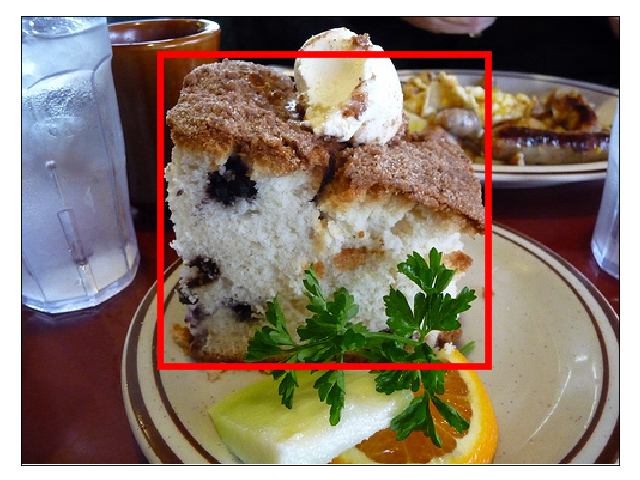
\includegraphics[scale=0.15]{figures/2390077_1254219_supercat_unique.png} &
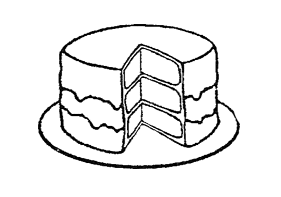
\includegraphics[scale=0.4]{figures/snodgrass_vanderwart_cake_042.png}\\
 cake\ (53),  food\ (19), bread\ (8), burger\ (6), dessert\ (6), snacks\ (3), muffin\ (3),  pastry\ (3) & \hspace{.9cm} cake (83)
\end{tabular}
\caption{Names for a cake object in ManyNames (left) and in Snodgrass's Naming Norms (right), percentages of responses in parentheses.}
\label{fig:cake}
\end{figure}


Here, for reasons of scope and space, we provide preliminary results on the amount and type of variation we find in the data.
%
The trends we identify in the dataset are illustrated in Figure \ref{fig:cake} (left): Our data reveals clear naming preferences (in the example, 53\% of the annotators prefer the name \word{cake}, corresponding to the so-called basic-level category, see Section~\ref{sec:rel-work}) and also rich variation (the remaining annotators prefer other options like \word{food, dessert, bread}) that is not restricted to taxonomic relations studied in previous work on naming \cite{Ordonez:2016,graf2016animal}: while \word{food} is in a taxonomic relation to \word{cake} (it is a hypernym), \word{dessert} highlights a different facet of the object.

%%% Local Variables:
%%% mode: latex
%%% TeX-master: "lrec2020naming"
%%% End:
